\documentclass[10pt,border=4pt]{standalone}
\usepackage{mathptmx}
\usepackage{amsmath,amssymb,bm}
\usepackage{tikz}
\usetikzlibrary{patterns,decorations.pathmorphing,decorations.pathreplacing,arrows.meta,fit,backgrounds,calc,positioning,shapes.geometric}
\definecolor{acc}{HTML}{0B5394}
\definecolor{accl}{HTML}{EAF0F7}
\definecolor{grp}{HTML}{F5F5F5}
\definecolor{org}{HTML}{C55A11}
\definecolor{orgl}{HTML}{FBEFE6}
\tikzset{
 dat/.style={draw=black,line width=0.6pt,fill=white,align=center,font=\small,inner sep=3pt,minimum height=0.85cm},
 lay/.style={draw=acc,line width=0.8pt,fill=accl,rounded corners=2pt,align=center,font=\small,inner sep=3pt,minimum height=0.85cm},
 cnd/.style={draw=org,line width=0.8pt,fill=orgl,rounded corners=2pt,align=center,font=\small,inner sep=3pt,minimum height=0.75cm},
 op/.style={circle,draw=black,line width=0.6pt,fill=white,inner sep=0.5pt,font=\small,minimum size=5mm},
 grpb/.style={draw=black!45,dashed,line width=0.6pt,rounded corners=3pt,inner sep=6pt},
 arr/.style={-{Latex[length=2.2mm,width=1.7mm]},line width=0.7pt},
 carr/.style={-{Latex[length=2.2mm,width=1.7mm]},line width=0.7pt,draw=org},
 shp/.style={font=\scriptsize,text=black!70,inner sep=1pt},
 lab/.style={font=\footnotesize,inner sep=1pt},
 ttl/.style={font=\small\bfseries,inner sep=0pt,anchor=west}
}
\newcommand{\xh}{\mathbf{x}_h}\newcommand{\xf}{\mathbf{x}_f}

\begin{document}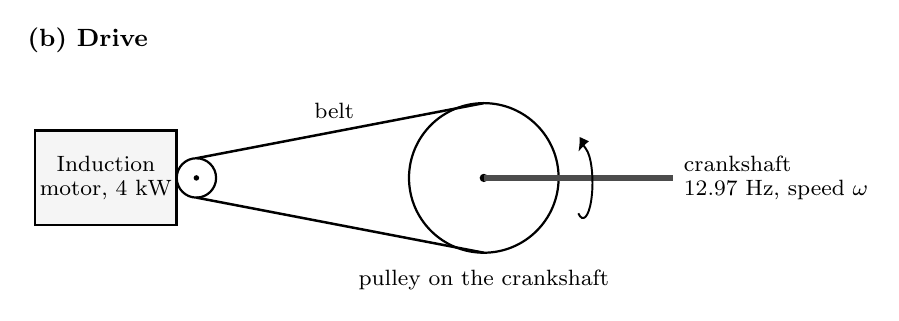
\begin{tikzpicture}[x=1cm,y=1cm]
\node[ttl] at (-0.6,1.75) {(b) Drive};
\draw[line width=0.9pt,fill=grp] (-0.5,-0.6) rectangle (1.3,0.6); \node[lab,align=center] at (0.4,0) {Induction\\[-1pt]motor, 4 kW};
\draw[line width=0.8pt,fill=white] (1.3,0) ++(0.25,0) circle (0.25); \fill (1.55,0) circle (1pt);
\draw[line width=0.8pt,fill=white] (5.2,0) circle (0.95); \fill (5.2,0) circle (1.5pt);
\draw[line width=0.9pt] (1.55,0.25)--(5.2,0.95) (1.55,-0.25)--(5.2,-0.95);
\node[lab] at (3.3,0.85) {belt};
\node[lab,align=center] at (5.2,-1.3) {pulley on the crankshaft};
\draw[line width=2.2pt,black!70] (5.2,0)--(7.6,0); \node[lab,anchor=west,align=left] at (7.7,0) {crankshaft\\[-1pt]12.97 Hz, speed $\omega$};
\draw[-{Latex[length=1.8mm]},line width=0.7pt] (6.4,-0.45) arc (-120:120:0.12 and 0.45);
\end{tikzpicture}\end{document}
